%   ------------------------------------------------------------------------
\FloatBarrier
\section{Análise do OpenArt.AI}
\label{s.openArt}

A ferramenta OpenArt AI foi selecionada para análise pela sua capacidade de edição de imagens por chat e geração de vídeos, agregando múltiplos modelos de IA para isso. A plataforma possui outros módulos interessantes (Figura \ref{fig:openArtModulos} no Apêndice \ref{ap.telasIA}) além dos que foram testados, como o módulo de personagem, que não pôde ser investigado pela limitação de créditos. Como base, todo usuário ao se cadastrar recebe 40 créditos grátis, sendo possível aumentar esse valor seguindo os canais da ferramenta em diferentes redes sociais.

O objetivo durante os testes foi gerar uma animação ou sprite do personagem Pablo sentado em front view, utilizando o sprite dele em pé como referência. O objeto onde o personagem se senta não deveria aparecer na imagem ou vídeo formado, pois a ideia era usar a mesma animação de sentar para qualquer objeto.

Primeiro, foi averiguado o módulo de vídeo, que fornecia diversas funcionalidades diferentes para a geração da animação (Figura \ref{fig:openArtModuloVideo} no Apêndice \ref{ap.telasIA}), porém só foi possível testar apenas uma delas. As funções que pareciam mais adequadas com o objetivo foram: Imagem para Vídeo e Elementos para Vídeo. Explorando melhor a interface e instruções das duas, foi escolhida a ferramenta de Elementos para Vídeo, porque a outra não permitia o uso de um prompt textual, criando um vídeo apenas com a imagem anexada sem nenhuma instrução.

A ferramenta permitia anexar até 7 elementos para o vídeo, todavia apenas o sprite do personagem foi anexado para não aparecer nenhum outro objeto em cena. Havia dois modelos de IA disponíveis para uso, Vidu Q1 e Kling 1.6 (Figura \ref{fig:openArtModelosVideo} no Apêndice \ref{ap.telasIA}). Analisando as opções, o Vidu Q1 foi considerado o mais adequado, pois o outro era mais especializado para fotorrealismo. Foi utilizado um prompt descrevendo como deveria ser a animação de sentar em detalhes, que pode ser consultado no Quadro \ref{quad:openArtPrompt}. A tela para geração do vídeo pode ser consultada na Figura \ref{fig:openArtVideo} no Apêndice \ref{ap.telasIA}.

\begin{figure}[htbp]
    \centering
    \captionof{quadro}{Prompt textual detalhado para geração de vídeo no OpenArt.AI.}
    \label{quad:openArtPrompt}
    \fbox{                                  % Este comando cria uma caixa ao redor do texto
        \begin{minipage}{0.9\textwidth}     % Define a largura da caixa de texto
            \vspace{1ex}                    % Adiciona um pequeno espaço no topo
            \textit{Create a 2D pixel art animation using the provided character. The animation should show the character moving from his current standing pose into a sitting position. Crucially, he is sitting on an object, like a chair or a couch. The animation frames should depict him bending his knees, lowering his hips, and leaning back slightly until he settles into a natural, relaxed sitting posture, suspended in mid-air. His final pose should look like he is being comfortably supported by something. Maintain the exact pixel art style, colors, and design of the character throughout the entire animation.}
            
            \vspace{2ex}                    % Adiciona um espaço entre o original e a tradução
            
            \noindent\textbf{Tradução livre:} Crie uma animação 2D em pixel art usando o personagem fornecido. A animação deve mostrar o personagem se movendo de sua pose atual em pé para uma posição sentada. Crucialmente, ele está sentado em um objeto, como uma cadeira ou um sofá. Os quadros da animação devem retratá-lo dobrando os joelhos, baixando os quadris e inclinando-se ligeiramente para trás até que ele se acomode em uma postura sentada natural e relaxada, suspenso no ar. Sua pose final deve parecer que ele está sendo confortavelmente apoiado por algo. Mantenha o estilo de pixel art, cores e design exatos do personagem durante toda a animação.
            \vspace{1ex}                    % Adiciona um pequeno espaço na base
        \end{minipage}
    }
    
    \legend{\small Fonte: Elaborada pela autora.}
\end{figure}

O resultado \footnote{\url{https://drive.google.com/file/d/1tCKdj0FJEHVoq5y0V6qRCAkA7e2ZNrcz/view?usp=sharing}} gerado foi insatisfatório, fazendo uma animação 3D onde o personagem é rotacionado e mexe a cabeça para cima antes de sentar em side view. O movimento de sentar também não é muito preciso, onde é parada a movimentação no meio por alguns momentos, para depois o personagem se agachar completamente, alguns segundos depois movendo as pernas para frente e para baixo do nível inicial do chão. Apesar disso, a ferramenta foi capaz de manter as características físicas consistentes e permitiu a exportação em gif. A Figura \ref{fig:openArtVideoFrames} apresenta frames da animação gerada.

\begin{figure}[htbp]
    \centering
    \caption{\small Frames do vídeo gerado no OpenArt.AI}
    \label{fig:openArtVideoFrames}
    \begin{subfigure}{0.45\linewidth}
    \centering
        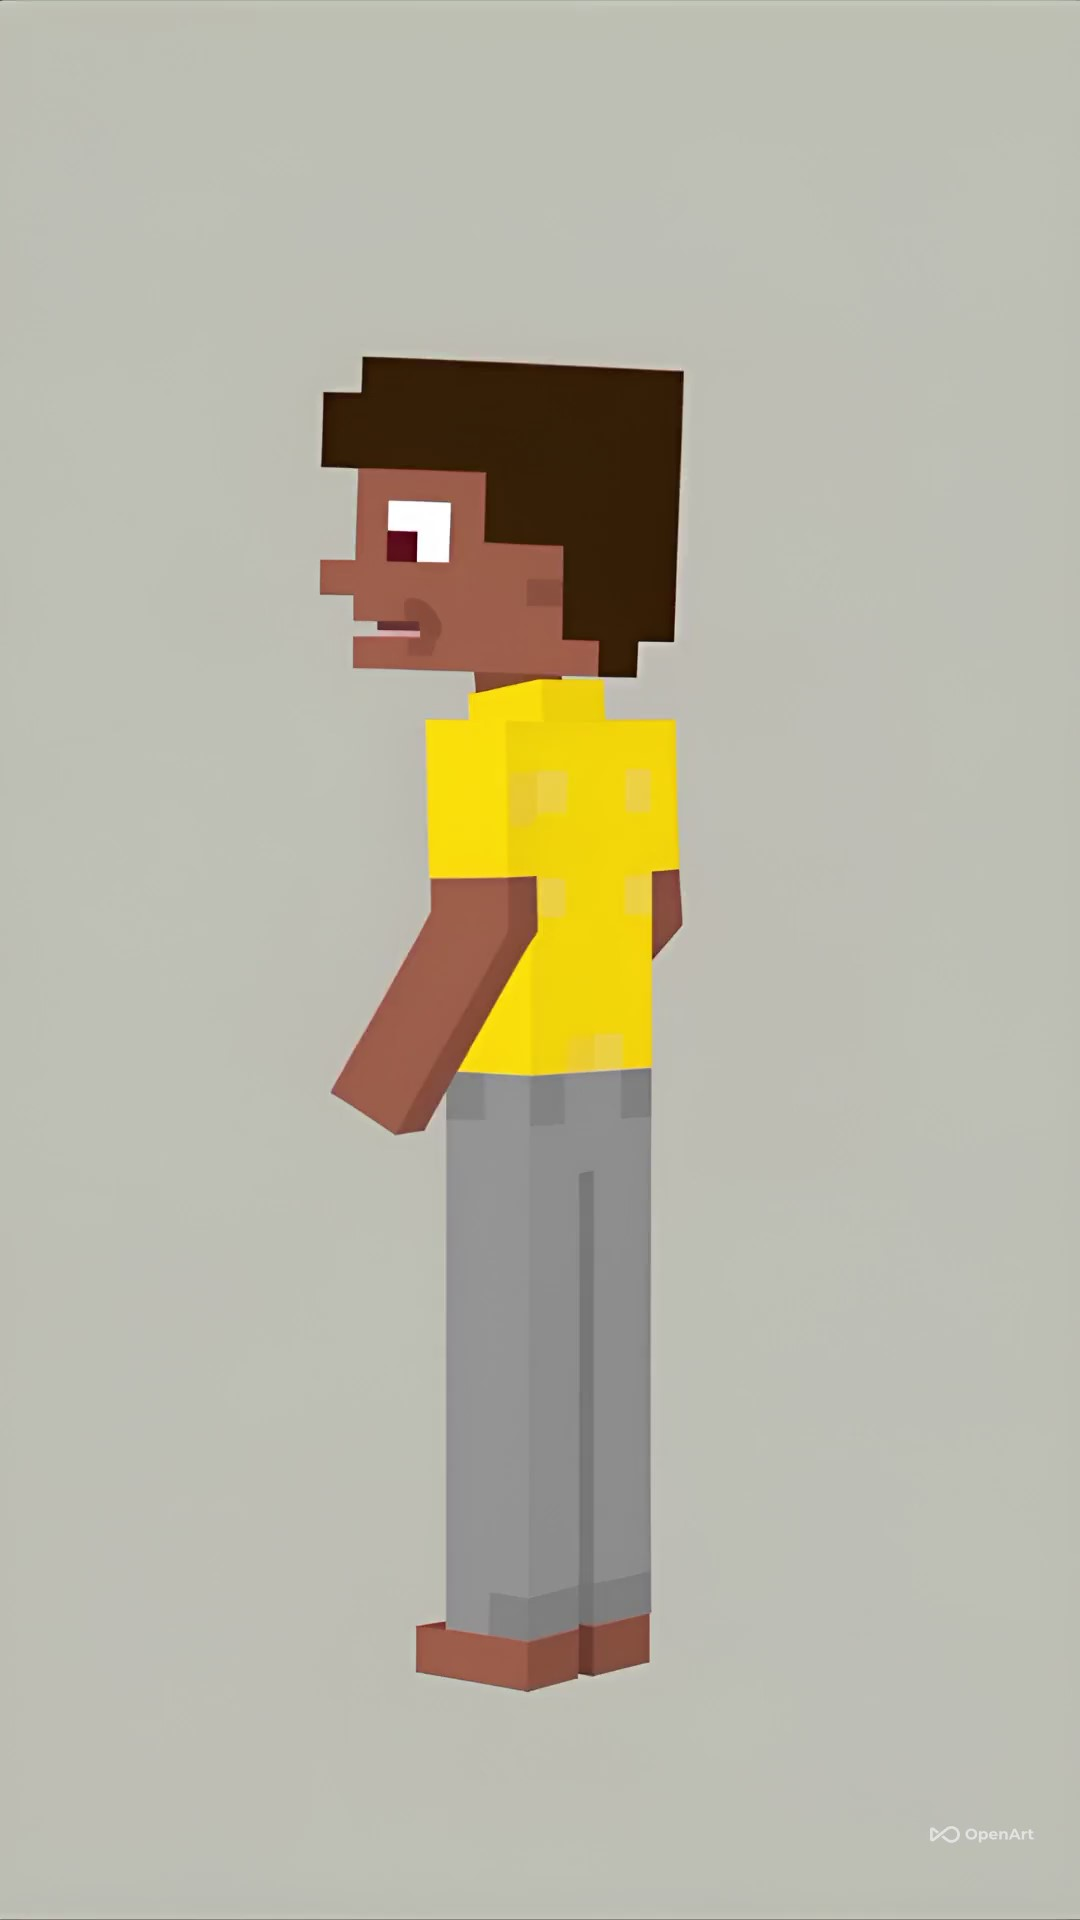
\includegraphics[width=0.65\linewidth]{figs/OpenArtAI/frame1.jpg}
        \caption{\small Primeiro frame}
        \label{fig:openArtVideoFrames1}
    \end{subfigure}
    \begin{subfigure}{0.45\linewidth}
    \centering
        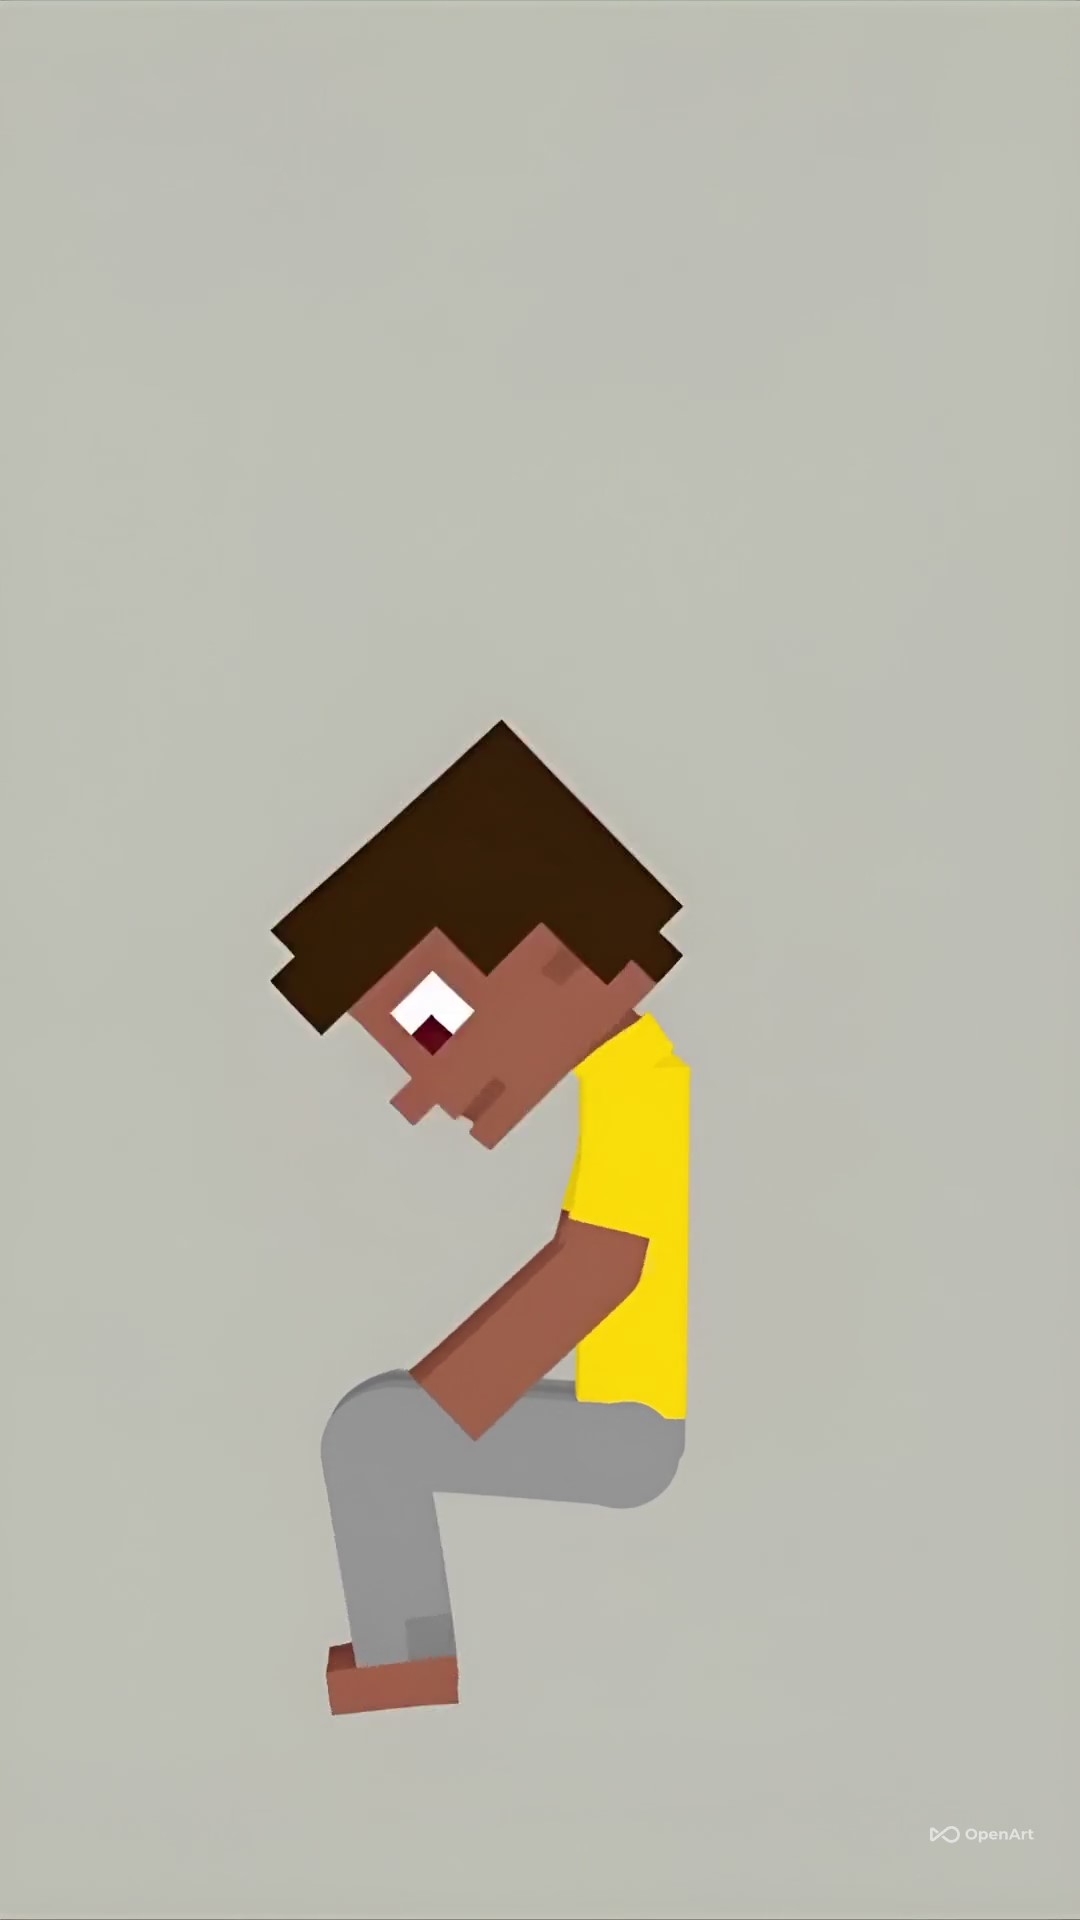
\includegraphics[width=0.65\linewidth]{figs/OpenArtAI/frame2.jpg}
        \caption{\small Último frame}
        \label{fig:openArtVideoFrames2}
    \end{subfigure}
    \legend{\small Fonte: Elaborada pela autora, utilizando a ferramenta OpenArt.AI.}
\end{figure}

Devido à geração do vídeo não ser bem-sucedida, os próximos testes focaram na geração de apenas o sprite do personagem sentado. Explorando o módulo de imagem, havia diversas funcionalidades (Figura \ref{fig:openArtModuloImagem} no Apêndice \ref{ap.telasIA}), porém apenas duas delas se mostraram acessíveis e adequadas para a análise: criar imagem e chat para editar. Foi escolhida a funcionalidade de chat para editar, pois em tese a consistência do personagem seria garantida.

A ferramenta de chat para editar apresentava várias opções de modelo de IA (Figura \ref{fig:openArtModelosImagem} no Apêndice \ref{ap.telasIA}) com diferentes níveis de geração. Uma interação com cada modelo foi realizada, visando editar o personagem em pé para a posição de sentado. Foi utilizado o mesmo prompt para os testes com diferentes modelos.

O modelo SeeEdit parece estar escrito de forma incorreta na plataforma. Durante pesquisas, não foi possível encontrar um modelo com esse nome específico, apenas outro extremamente similar chamado SeedEdit 3.0 da BytePlus. O logo da empresa BytePlus coincidiu com o logo ao lado do SeeEdit no OpenArtAI, o que concretiza a hipótese do erro de digitação. O SeedEdit é um modelo de edição de imagens através de instruções de texto, se destacando em modificar áreas-chave com precisão, mantendo outras informações detalhadas com alta consistência \cite{modelark-byteplus_2025}. O resultado gerado foi satisfatório, sem mudar nenhuma região desnecessária do personagem, mantendo a característica e proporção da perna e mantendo o ambiente em 2D, porém perdendo a característica do estilo de pixel art na área específica modificada. Essa incongruência não chamou tanta atenção pois ainda se manteve o estilo simples, inclinando o que reto parecia formar uma pixel art, e as duas curvas realizadas não ficaram destoantes. É possível verificar isso na Figura \ref{fig:openArtSeedEdit}.

\begin{figure}[htbp]
    \centering
    \caption{\small Imagem gerada pelo modelo SeedEdit no OpenArtAI}
    \label{fig:openArtSeedEdit}
    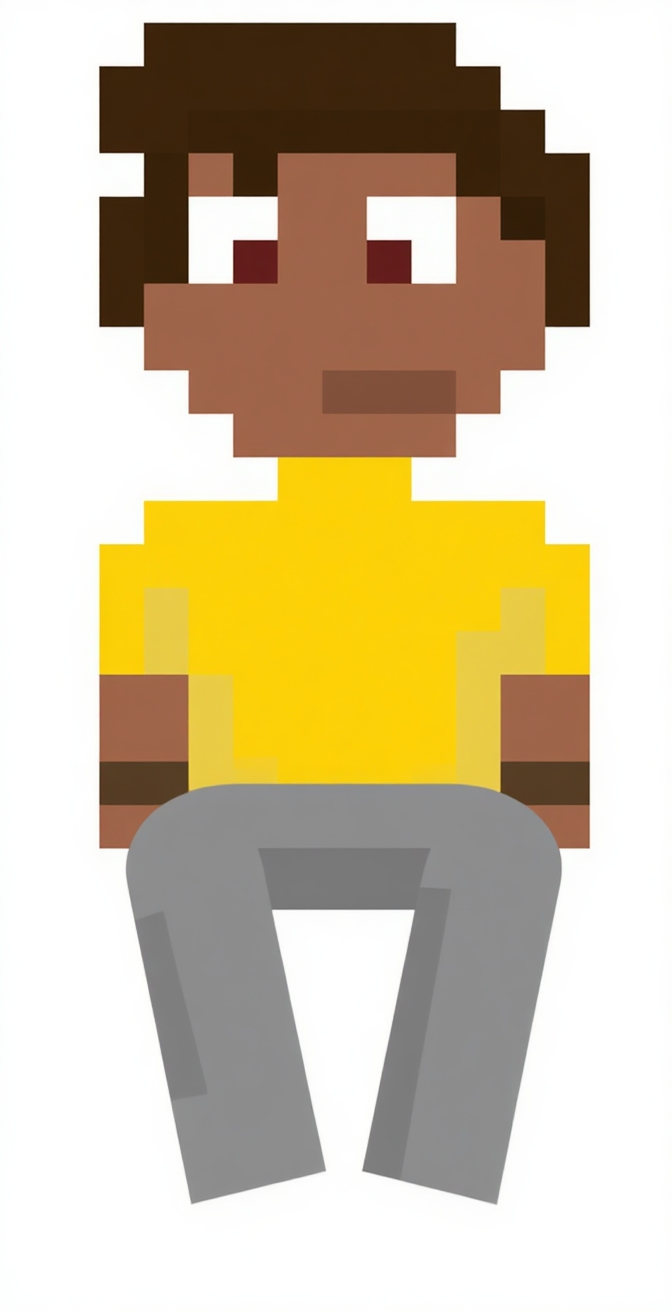
\includegraphics[width=0.2\linewidth]{figs/OpenArtAI/seeEdit.png}
    \legend{\small Fonte: Elaborada pela autora,utilizando a ferramenta OpenArt.AI.}
\end{figure}

O Flux Kontext é uma família de modelos que utilizam o método flow matching (correspondência de fluxo, em inglês) para geração e edição de imagens. Diferente do modelo Flux, ele é capaz de entender imagens existentes e modificá-las de acordo com instruções de texto simples \cite{blackforestlabs_2025}. O resultado gerado foi quase satisfatório, mantendo o personagem e o estilo consistente, porém gerando a cadeira, adicionando um sapato cinza escuro e com uma perna mais grossa que a outra. A Figura \ref{fig:openArtFluxKontext} apresenta esse resultado.

\begin{figure}[htbp]
    \centering
    \caption{\small Imagem gerada pelo modelo Flux Kontext Pro no OpenArtAI}
    \label{fig:openArtFluxKontext}
    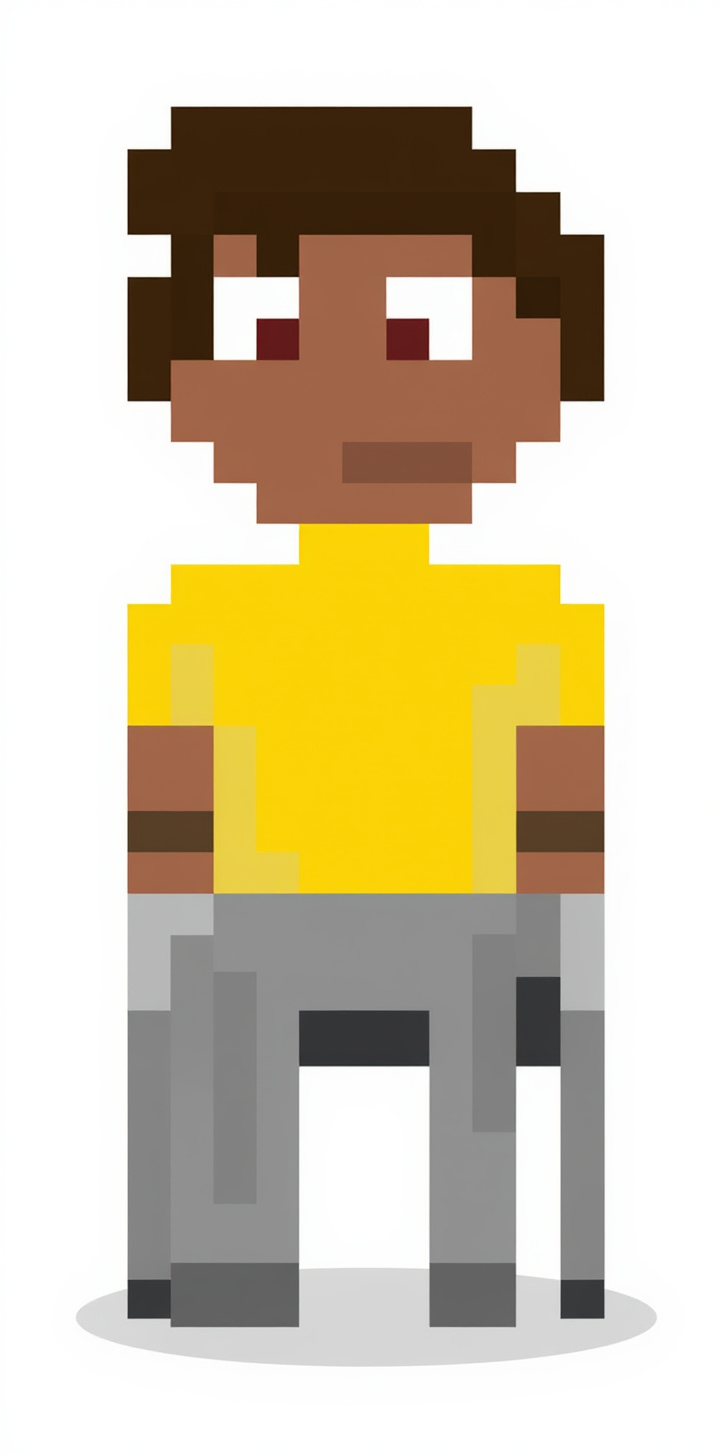
\includegraphics[width=0.2\linewidth]{figs/OpenArtAI/fluxKontextPro.png}
    \legend{\small Fonte: Elaborada pela autora,utilizando a ferramenta OpenArt.AI.}
\end{figure}

O Gemini é um modelo de IA capaz de entender, operar e combinar diversos tipos de dados, como texto e imagem \cite{sundarpichai_2023}. Porém, na plataforma OpenArt.AI não foi encontrada nenhuma informação específica sobre a versão do modelo. O resultado gerado não foi satisfatório, pois, apesar de manter a consistência, foi desenhada uma cadeira em outro estilo e ângulo, o personagem não foi bem encaixado no assento e os joelhos ficaram dobrados para cima. Imagem mostrada na Figura \ref{fig:openArtGemini}.

\begin{figure}[htbp]
    \centering
    \caption{\small Imagem gerada pelo modelo Gemini no OpenArtAI}
    \label{fig:openArtGemini}
    
\includegraphics[width=0.2\linewidth]{figs/OpenArtAI/gemini.png}
    \legend{\small Fonte: Elaborada pela autora,utilizando a ferramenta OpenArt.AI.}
\end{figure}

Testando o mesmo prompt diretamente no Gemini Pro, os resultados não foram melhores e continuou havendo problemas de precisão, como pode ser visto na Figura \ref{fig:openArtComparaGemini}.

\begin{figure}[htbp]
    \centering
    \caption{\small Imagens geradas pelo modelo Gemini}
    \label{fig:openArtComparaGemini}
    \begin{subfigure}{0.32\linewidth}
    \centering
        
\includegraphics[width=1\linewidth]{figs/OpenArtAI/gemini.png}
        \caption{\small Resultado gerado dentro do OpenArtAI}
        \label{fig:openArtComparaGemini1}
    \end{subfigure}
    \begin{subfigure}{0.32\linewidth}
    \centering
        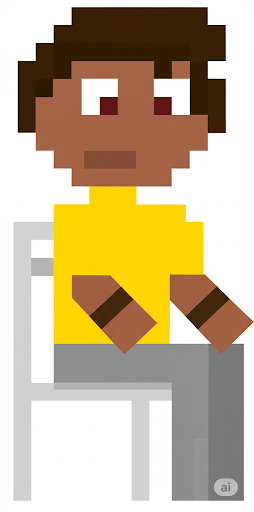
\includegraphics[width=0.8\linewidth]{figs/geminiPro/compararDalle3_res.PNG}
        \caption{\small Resultado 1 gerado dentro do Gemini Pro}
        \label{fig:openArtComparaGemini2}
    \end{subfigure}
    \begin{subfigure}{0.32\linewidth}
    \centering
        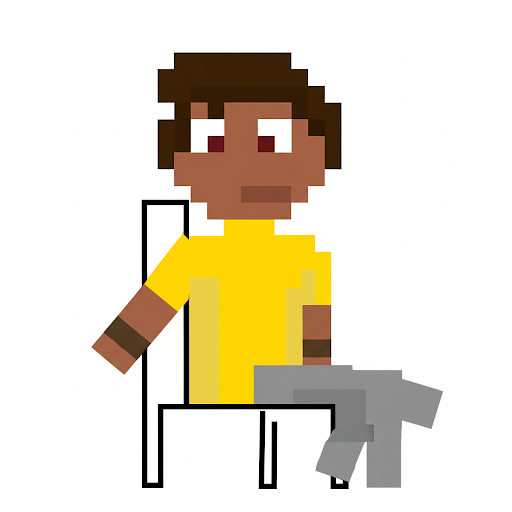
\includegraphics[width=1\linewidth]{figs/geminiPro/compararDalle3_res2.PNG}
        \caption{\small Resultado 2 gerado dentro do Gemini Pro}
        \label{fig:openArtComparaGemini3}
    \end{subfigure}
    \legend{\small Fonte: Elaborada pela autora, utilizando a ferramenta OpenArt.AI e Gemini Pro.}
\end{figure}

Diferente do ChatGPT, que é a aplicação de chatbot oficial da OpenAI, o GPT é o modelo utilizado, como já foi explicado na Seção \ref{s.chatGPT}. O resultado foi insatisfatório, alterando levemente os tons de cores e o tamanho do personagem, além de mudar o ângulo em 45 graus. Apesar disso, a imagem manteve o estilo de pixel art e as características em geral do personagem, não mostrando a cadeira. A Figura \ref{fig:openArtComparaGPT} compara o personagem original com o sprite gerado.

\begin{figure}[htbp]
    \centering
    \caption{\small Comparação do sprite original e do sprite gerado pelo modelo GPT no OpenArt.AI}
    \label{fig:openArtComparaGPT}
    \begin{subfigure}{0.45\linewidth}
    \centering
        
\includegraphics[width=0.5\linewidth]{figs/sprites/Pablo.PNG}
        \caption{\small Sprite original}
        \label{fig:openArtComparaGPTOriginal}
    \end{subfigure}
    \begin{subfigure}{0.45\linewidth}
    \centering
        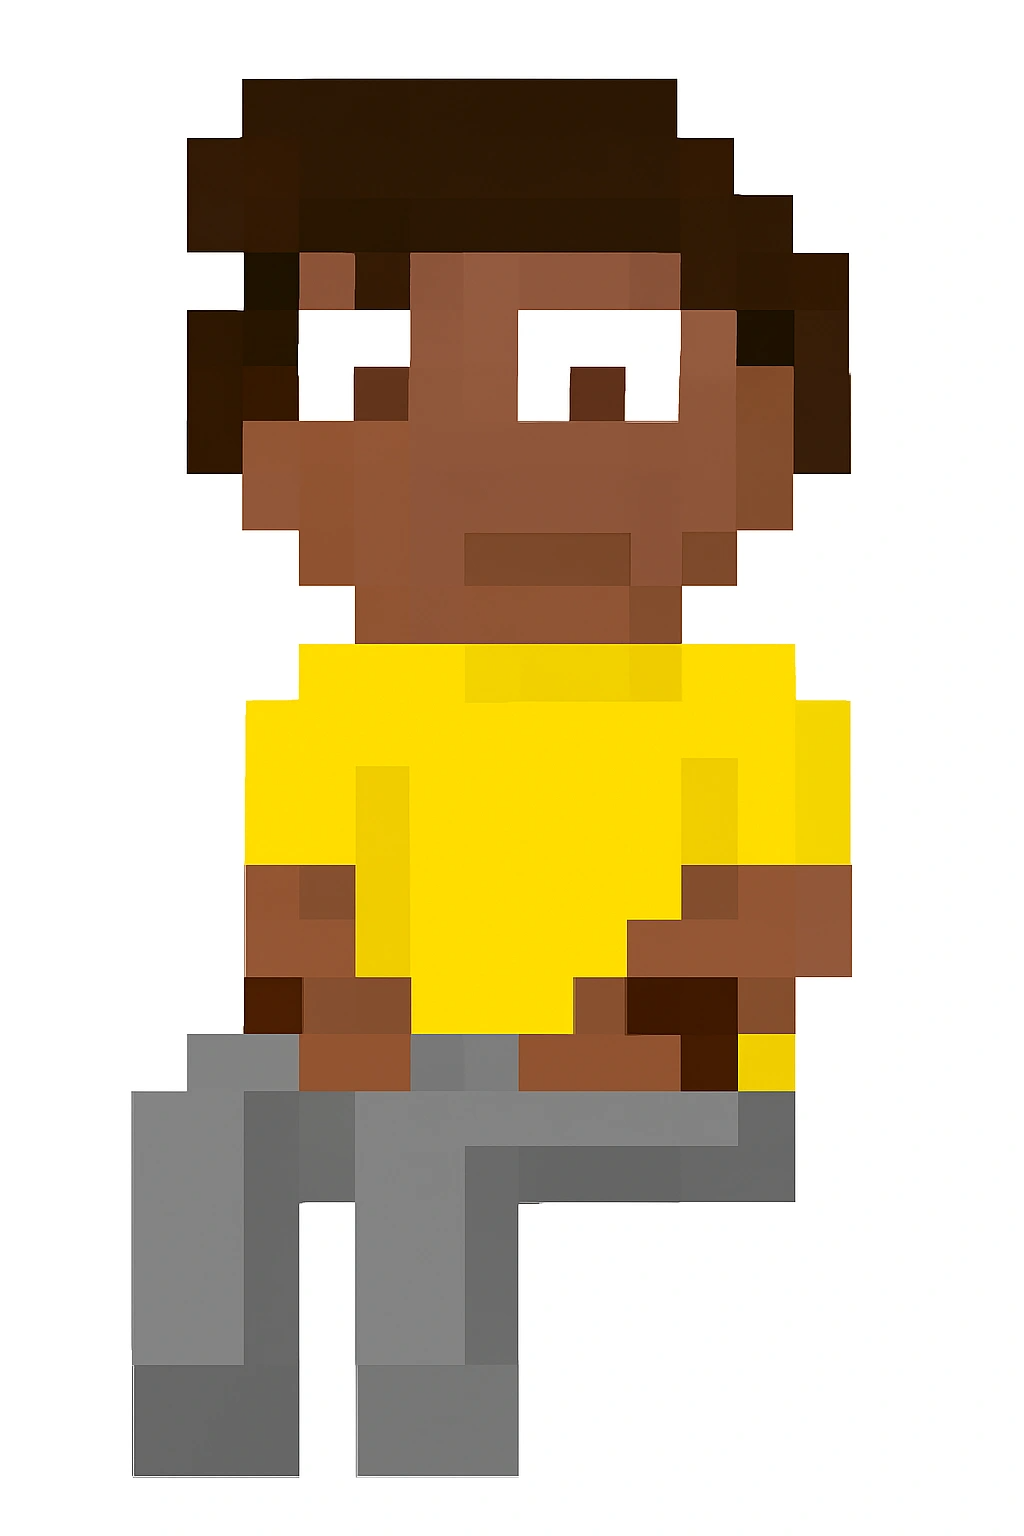
\includegraphics[width=0.5\linewidth]{figs/OpenArtAI/gpt.png}
        \caption{\small Resultado gerado pelo GPT no OpenArtAI}
        \label{fig:openArtComparaGPTGerado}
    \end{subfigure}
    \legend{\small Fonte: Elaborada pela autora, utilizando a ferramenta OpenArt.AI e Gemini Pro.}
\end{figure}


Todas as interações podem ser consultadas nas Figuras \ref{fig:openArtModeloSeedEdit} a \ref{fig:openArtModeloGPT} no Apêndice \ref{ap.telasIA}.

Apesar da animação gerada não ter sido satisfatória, o OpenArt.AI demonstrou grande potencial na edição de imagem, servindo como uma excelente ferramenta para a iteração de edições. Nenhum modelo individual foi capaz de gerar um resultado sem erros, porém deve-se notar que a análise foi limitada a uma única iteração por modelo devido à restrição de créditos. Funcionalidades de edição via chat são iterativas, projetadas para que o usuário aponte as falhas de uma geração e a IA as corrija em tentativas subsequentes. A impossibilidade de realizar este ciclo de refinamento pode ter impactado o desempenho final de cada modelo.

Apesar da animação gerada não ter sido satisfatória, o OpenArt.AI demonstrou grande potencial na edição de imagem, servindo como uma excelente ferramenta para a iteração e ideação de poses. Nenhum modelo individual foi capaz de gerar um resultado final sem erros, contudo, é fundamental ressaltar que a análise foi limitada a uma única iteração por modelo devido à restrição de créditos. Funcionalidades de edição via chat são inerentemente iterativas, projetadas para que o usuário aponte as falhas de uma geração e a IA as corrija em tentativas subsequentes. A impossibilidade de realizar este ciclo de refinamento pode ter impactado o desempenho final de cada modelo.

%tentei iteração com gemini, e ficou melhor do que o primeiro resultado da iteração nova, mas foi meio esquisito como se comportou